\documentclass{article}

\usepackage{dibrisunige-report}
\usepackage{codespace}
\usepackage{seqsplit}
\usepackage{longtable}

% Sub-preambles
% https://github.com/MartinScharrer/standalone

% Encodings
\usepackage{amsmath,amssymb,gensymb,textcomp}

% Better tables
% Wide tables go to https://tex.stackexchange.com/q/332902
\usepackage{array,multicol,multirow,siunitx,tabularx}

% Better enum
\usepackage{enumitem}

% Graphics
\usepackage{caption,float}

% Allow setting >max< width of figure
% 'export' allows adjustbox keys in \includegraphics
\usepackage[export]{adjustbox}

% For demonstration purposes, remove in production
\usepackage{mwe}

% Configurations
\newcounter{memberrowno}
\setcounter{memberrowno}{0}
\setlength{\headheight}{32pt}
\ocoursename{Augmented and Virtual Reality - code 80459 - a.y. 2025/2026}
\oreporttype{Final Report}
\otitle{Extending Cosys-AirSim for  Multi-Domain Vehicle Simulation}
\osubtitle{\textit{Bringing Aerial and Ground Robotics Together in One Simulation}}
\oadvisor{Manuel Delucchi, Saverio Iacono, Gianni Viardo Vercelli}
\ostudent{Andrea Valentino Ricotti, Walter Signoretti, Azzurra Suffia}
\reportlayout%

% Custom commands
\newcommand*\mean[1]{\bar{#1}}

% Title and Metadata
\title{Extending Cosys-AirSim for  Multi-Domain Vehicle Simulation}
\author{Andrea Valentino Ricotti, Walter Signoretti, Azzurra Suffia}
\date{\today}

\begin{document}
% Cover Page
\coverpage%

\section*{Member list \& Workload}
\begin{center}
  \begin{tabular}{>{\stepcounter{memberrowno}\thememberrowno}llcc}
    \toprule
    \multicolumn{1}{c}{\textbf{No.}} & \textbf{Full name} & \textbf{Student ID} & \textbf{Percentage of work} \\
    \midrule
                                     & Andrea Valentino Ricotti      & 5306194             & 100\%                       \\
                                     & Walter Signoretti             & 5240038             & 100\%                       \\
                                     & Azzurra Suffia                & 5341007             & 100\%                       \\
    \bottomrule
  \end{tabular}
\end{center}

\newpage

\begin{abstract}
\noindent
We enhanced Cosys-Airsim, an Unreal Engine plugin based on Microsoft AirSim, by implementing support for diverse, multi-vehicle fleets. 
Previously limited to single-type setups, our modification enables concurrent interactions between diverse vehicles like UAVs and UGVs. 
By assigning unique server ports to each vehicle and introducing new logic classes, we facilitate complex, multi-modal simulation scenarios formerly unsupported by the platform.
\end{abstract}

\newpage

% Table of Contents
\tableofcontents

\newpage

\section{Introduction}
\subsection{State of Art}
\noindent
The field of robotics has witnessed a significant paradigm shift from single-agent missions to complex Multi-Robot Systems (MRS) and Heterogeneous Multi-Agent Systems (MAS). 
Research in this area, which dates back to the late 1980s \cite{cao1997cooperative}, has demonstrated that coordinated teams of robots can achieve mission objectives that are beyond the capabilities of individual units. 
Heterogeneous systems, characterized by agents with diverse physical structures and capabilities, offer enhanced fault tolerance, scalability, and the ability to perform multi-faceted tasks through the fusion of multi-modal data.\newline\newline
The integration of Unmanned Aerial Vehicles (UAVs) and Unmanned Ground Vehicles (UGVs) is a prominent example of such synergy. While UAVs provide rapid exploration and global situational awareness from an aerial perspective, UGVs contribute with extended endurance, higher payload capacities, and stable interaction with the ground environment. 
This collaborative approach has found critical applications in structural monitoring of historical infrastructure, as well as in Search and Rescue (SAR)~\cite{HUANG2024109491}, industrial inspection~\cite{s20216384} and precision agriculture tasks.\newline\newline
Despite its potential, UAV-UGV collaboration faces significant scientific challenges~\cite{munasinghe2024uavugv}, particularly in optimizing communication and coordination under unstable network conditions. Recent research has explored solutions like the Unified Robotic Protocol (URP) to manage communication between diverse frameworks \cite{shahar2025ugv_uav}, and resource-efficient strategies like Semantic Communication (SemCom) \cite{zhang2023semantic}, which prioritizes the transmission of task-relevant semantic information over raw data to reduce bandwidth overhead.\newline\newline
The complexity of these systems necessitates high-fidelity simulation environments for safe and cost-effective validation. While traditional tools like Gazebo and Webots provide robust physics-based simulation, they often lack the photorealistic rendering required for advanced vision-based perception algorithms. In this context, simulators built on high-performance game engines, such as Microsoft's AirSim \cite{airsim}, have become state-of-the-art by offering realistic environmental physics and sensor behavior, as highlighted in recent comparative reviews \cite{nikolaiev2024comparative}.\newline\newline
Building upon this foundation, Cosys-AirSim~\cite{jansen2023cosys} was developed to address specific industrial and research needs, including more detailed sensor models and procedurally generated environments. However, a persistent limitation in existing frameworks, including the baseline AirSim implementation, is the lack of support for heterogeneous multi-vehicle configurations in unified scenes.
The proposed project addresses this gap by extending the Cosys-AirSim architecture to support concurrent interaction and control of UAVs and UGVs. This enhancement facilitates the integrated testing of perception and coordination strategies, positioning the platform as a leading tool for multi-domain autonomous research in immersive and virtual environments.


\subsection{Motivation}
\noindent
This project aims to extend \textbf{Cosys-AirSim}, an open-source framework built upon Microsoft's AirSim simulator, which provides high-fidelity, physics-based environments for autonomous vehicles. 
While the current framework offers robust tools for simulating either Unmanned Aerial Vehicles (UAVs) or Unmanned Ground Vehicles (UGVs), it is restricted to single-domain operations, forcing users to choose only one vehicle type per simulation instance.
The current inability of Cosys-AirSim to support concurrent UAV and UGV simulation creates a bottleneck for researchers and industries needing to validate multi-domain systems in a unified virtual space.
\begin{figure}[H]
\centering
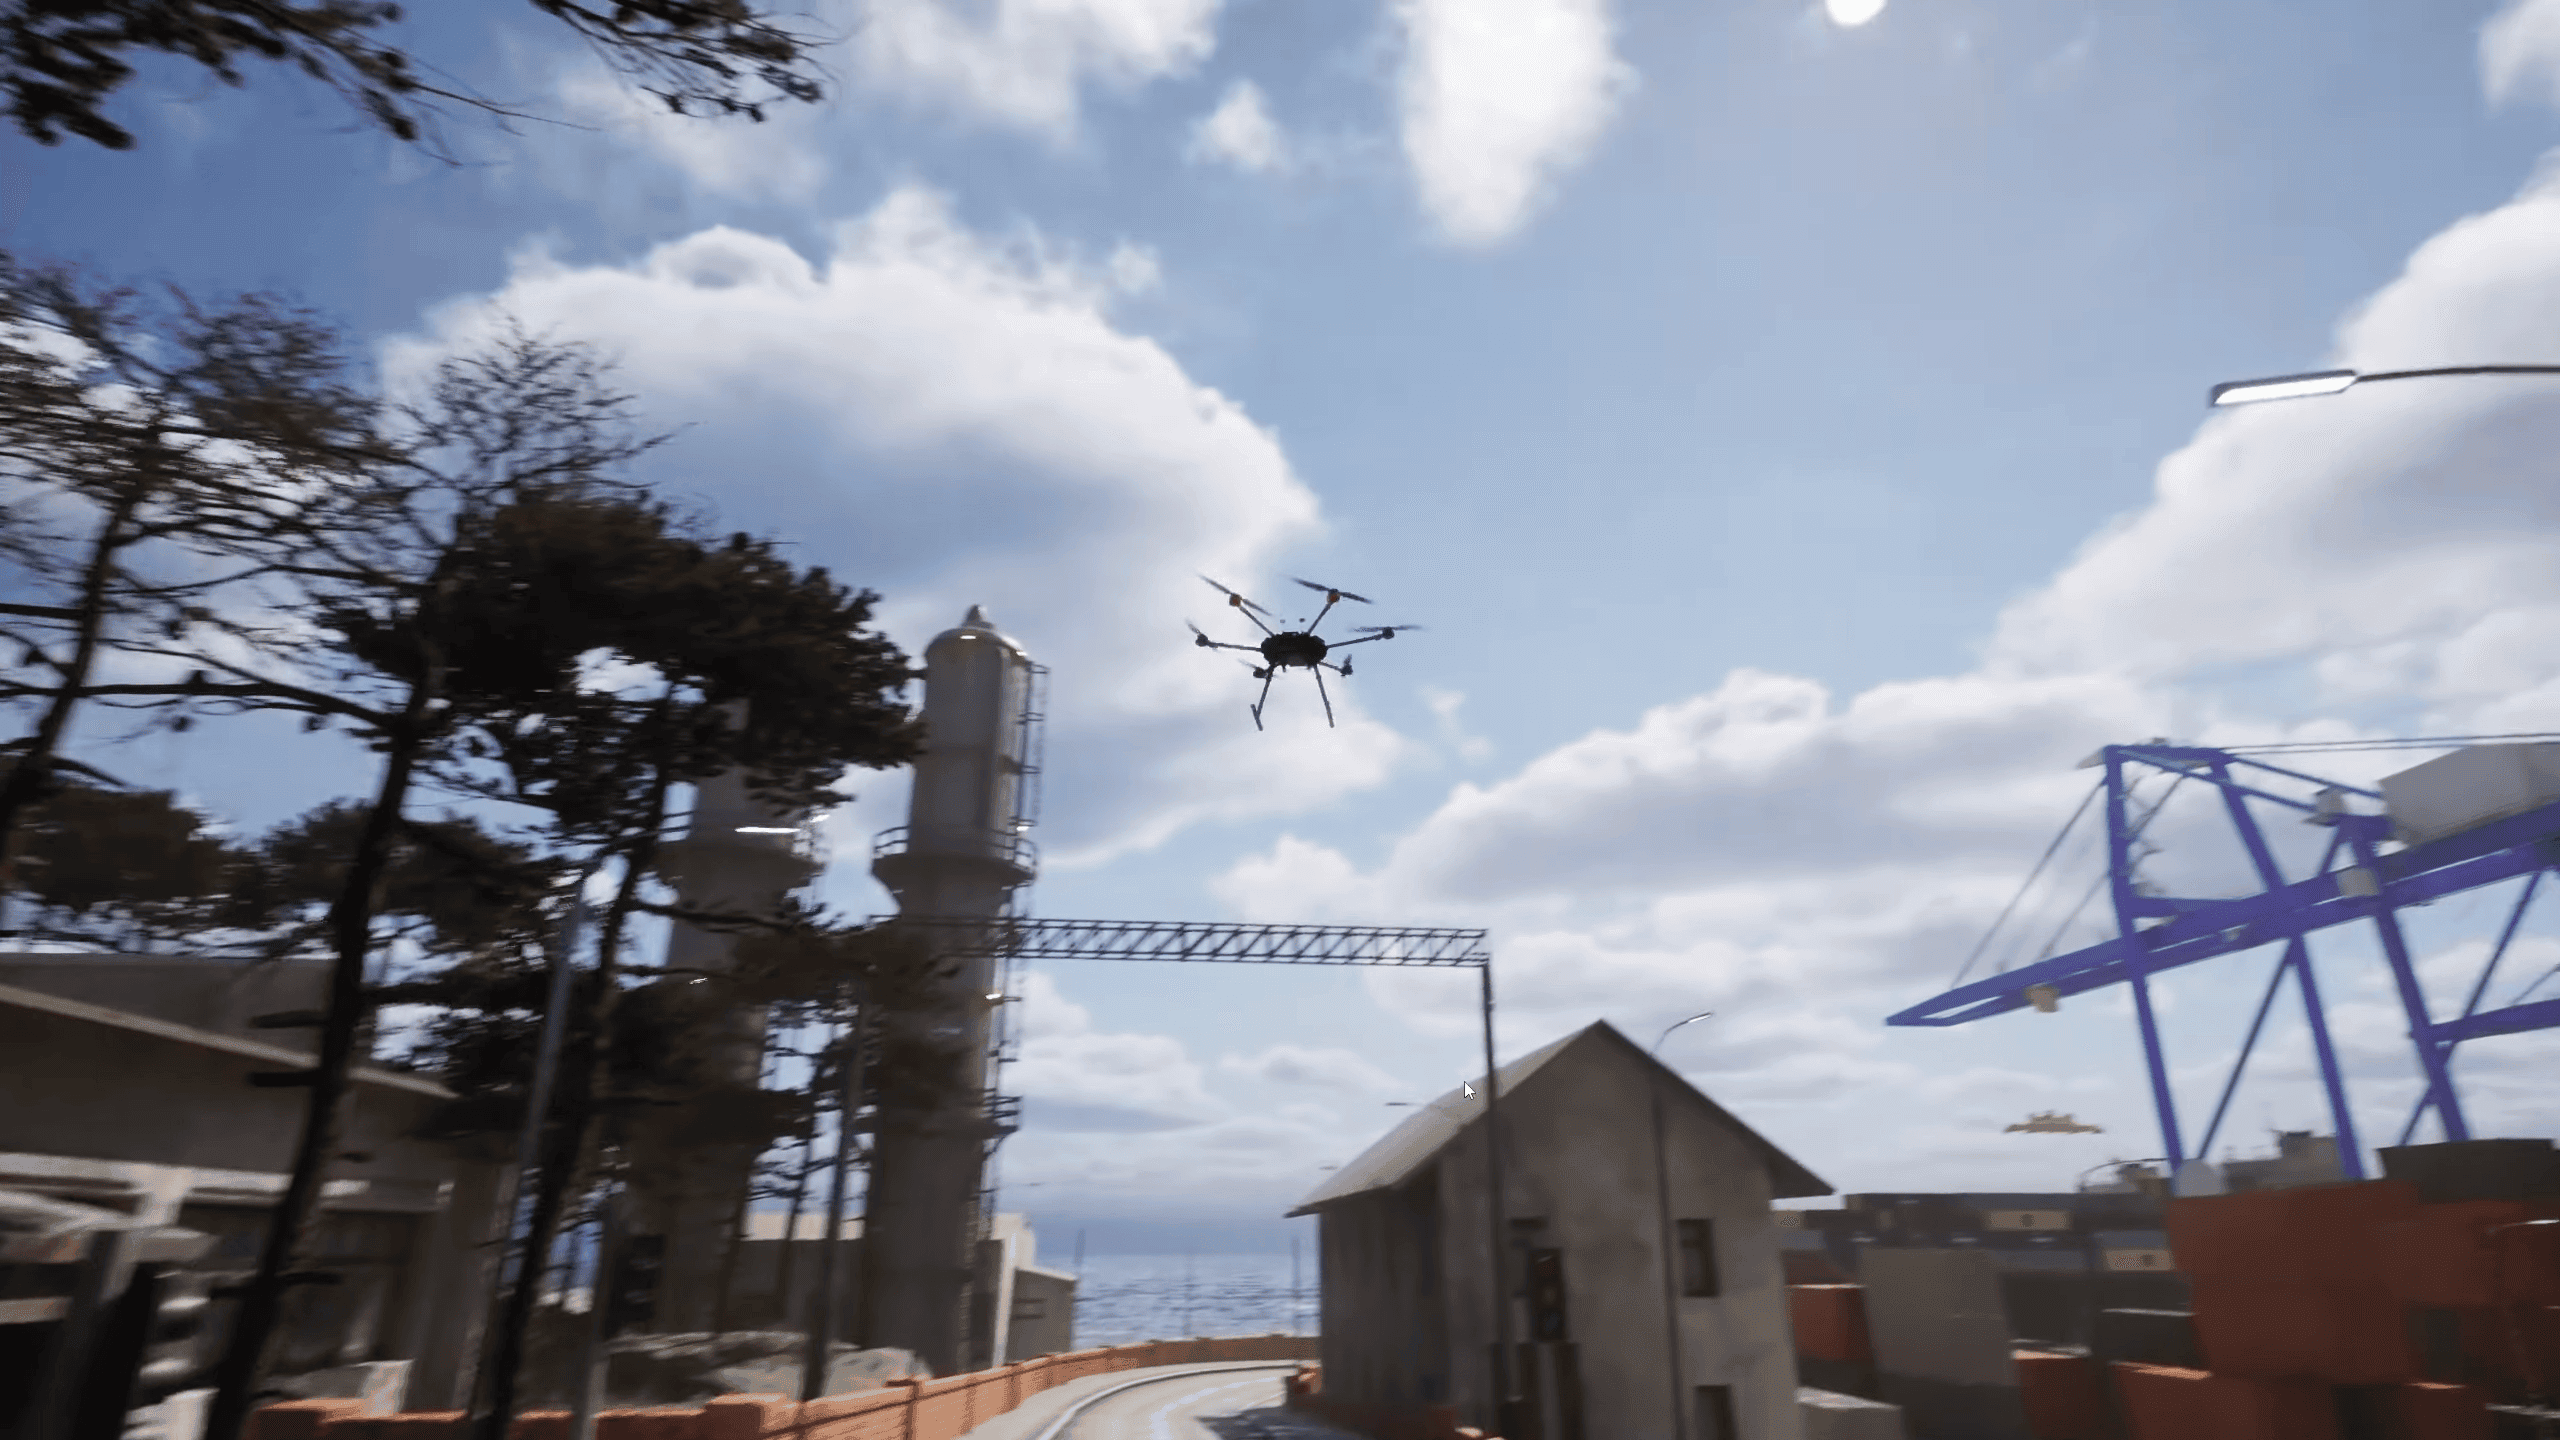
\includegraphics[width=0.4\textwidth]{graphics/Cosys_Airsim_UAV_example.png}
\caption{Example view of a UAV produced by Cosys-AirSim.}
\label{fig:UAV_example_view}
\end{figure}
\begin{figure}[H]
\centering
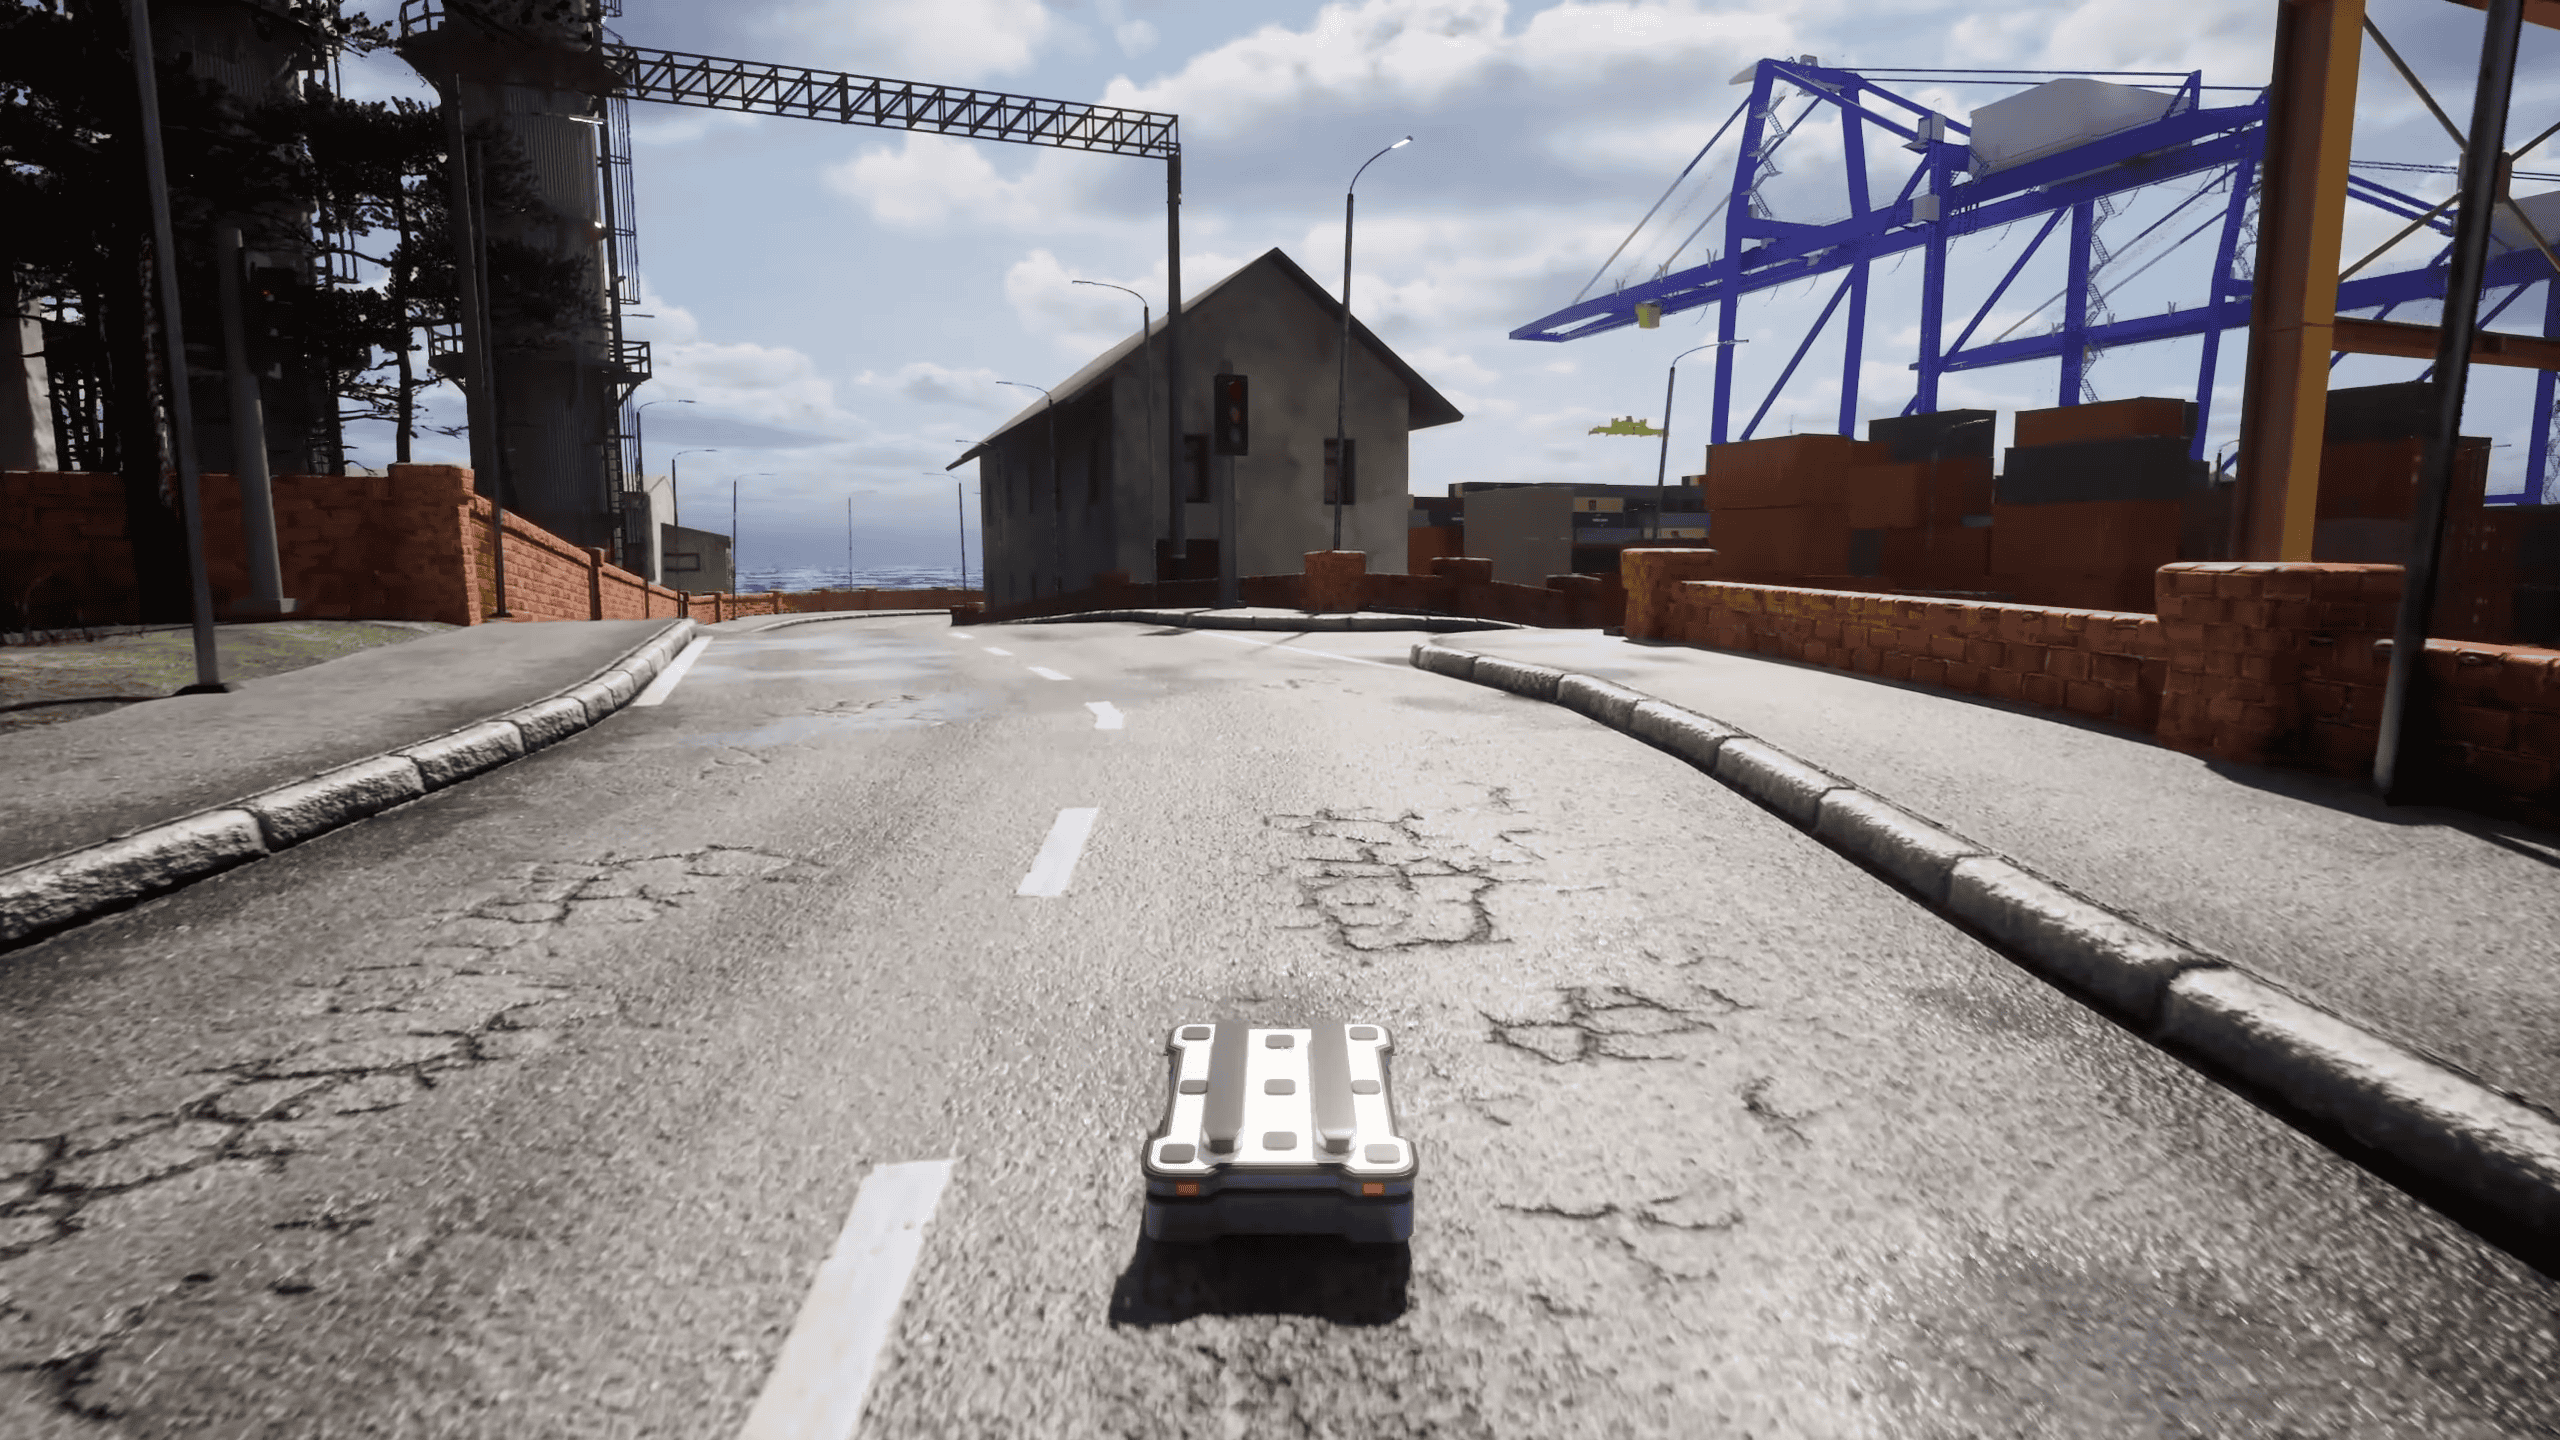
\includegraphics[width=0.4\textwidth]{graphics/Cosys_Airsim_UGV_example.png}
\caption{Example view of a UGV produced by Cosys-AirSim.}
\label{fig:UGV_example_view}
\end{figure}
\noindent
By modifying the underlying architecture to support simulations involving different vehicle domains simultaneously, this project seeks to bridge the gap between simulation and real-world cross-domain deployment. Furthermore, as an extension of an open-source tool, this work contributes to the broader robotics community by providing a flexible, accessible platform for testing cooperative strategies, ultimately reducing the risks and costs associated with physical multi-robot experimentation.


\subsection{AirLib, AirSim \& Cosys-AirSim}
\noindent
To fully grasp the scope of this extension, it is necessary to understand the underlying architecture of the simulation ecosystem and the specific differences between AirLib, AirSim~\cite{airsim}, and Cosys-AirSim~\cite{jansen2023cosys}.

\begin{itemize}
    \item \textbf{AirLib:} This is the foundational, engine-independent C++ library that serves as the core "brain" of the simulator. It handles the underlying physics, vehicle dynamics, and external API communications, functioning completely independently of the visual rendering engine.
    
    \item \textbf{AirSim:} Originally developed by Microsoft Research, AirSim is the complete open-source framework that encapsulates AirLib and bridges it with Unreal Engine via dedicated plugins. However, Microsoft has officially archived the open-source repository, ceasing further updates and leaving the original framework incompatible with newer technologies.
    
    \item \textbf{Cosys-AirSim:} To keep the project alive and modernize its capabilities, Cosys-Lab created Cosys-AirSim as a direct fork of the original AirSim. Beyond simply maintaining the code, Cosys-Lab significantly extended the framework by migrating it to Unreal Engine 5, enhancing the sensor suite, and improving overall fidelity. However, like its predecessor, it still has the limitation of only supporting a single vehicle domain per simulation session.
\end{itemize}

\newpage

\section{System Configuration \& Hardware Requirements}
\label{sec:requirements}
\subsection{Hardware Requirements}
\noindent
To ensure the high-fidelity physics and graphical rendering of the Cosys-AirSim ecosystem, the following hardware specifications are recommended for all users:

\begin{itemize}
    \item \textbf{Processor:} x86-64 architecture (although UE5.1+ supports ARM).
    \item \textbf{Memory:} A minimum of 8\,GB RAM is required, though 16\,GB is strongly recommended.
    \item \textbf{Storage:} At least 100\,GB of available disk space is recommended to accommodate the full ecosystem, including Unreal Engine, the simulator, and development tools.
    \item \textbf{Graphics:} A dedicated GPU is necessary to support high graphical settings and maintain the frame rates required for accurate real-time sensor simulation.
\end{itemize}

\subsection{Software Prerequisites}
\noindent
The software environment is primarily optimized for Windows to ensure full compatibility with simulation and debugging tools. Requirements vary depending on whether the user intends to modify the source code:

\begin{itemize}
    \item \textbf{Operating System:} Windows 11 is the preferred platform. While Ubuntu is supported for execution, it is not recommended for core development as it lacks support for the Visual Studio IDE.
    \item \textbf{Simulation Engine:} The required simulation environment consists of Unreal Engine 5.5 and the Cosys-AirSim v3.3 framework.
    \item \textbf{Integrated Development Environment (for Developers):} Visual Studio 2022 is the suggested IDE. Note that installing Unreal Engine and attempting to create a project will typically prompt the user to install Visual Studio Community 2022 if it is not already present.
    \item \textbf{Version Control (for Developers):} Git and GitHub are required for source code management and collaborative contributions.
    \item \textbf{Programming Languages:} While Python and C++ are both used for vehicle control and API interaction, framework modifications strictly require C++.
\end{itemize}\newpage

\section{Cosys-AirSim}

\subsection{Overview}
\noindent
An Unreal Engine plugin is a modular collection of code and data that extends the engine's core functionality. In general, these plugins are installed by placing the plugin folder into the \texttt{Plugins} directory of a specific project, allowing the engine to recognize and load the additional features upon startup.

\subsection{Installation \& Configuration}
\noindent
The following step-by-step guide assumes the software and hardware prerequisites discussed in Section~\ref{sec:requirements} and uses the \texttt{Blocks} environment provided by the official Cosys-AirSim documentation as the base project; however, it remains applicable to any Unreal Engine 5.5 environment.

\begin{enumerate}[label=\textbf{Step \arabic*:}, leftmargin=*]
    \item \textbf{Install Cosys-AirSim:} The plugin installation instructions are provided by the \href{https://cosys-lab.github.io/Cosys-AirSim/install_windows/}{official documentation}. 
    
    \item \textbf{Set up the Environment:} For the \texttt{Blocks} environment, follow the \href{https://cosys-lab.github.io/Cosys-AirSim/unreal_blocks/}{instructions} provided. Optionally, navigate to the \texttt{\seqsplit{Cosys-AirSim/Unreal/Environments}} directory and copy the \texttt{Blocks} folder to your desired working directory; this folder will serve as the primary Unreal Engine project.
    
    \item \textbf{Integrate the Extended Plugin:} Ensure that the \texttt{AirSim} folder is present within your project's \texttt{Plugins} directory. Otherwise, copy and paste the folder from the material downloaded in Step 1 into this directory.
    
    \item \textbf{Workspace Cleanup:} To ensure a clean build, delete the following temporary directories if they exist in both the root folder and the \texttt{\seqsplit{Plugins/AirSim}} folder: \texttt{Binaries}, \texttt{Intermediate}, \texttt{Saved}, and \texttt{DerivedDataCache}.
    
    \item \textbf{Project Compilation:} You may compile the project using one of two methods:
    \begin{itemize}
        \item \textbf{Visual Studio:} Right-click the \texttt{\seqsplit{Blocks.uproject}} file, select \textit{Generate Visual Studio project files}, open the resulting \texttt{.sln} file, and build the solution in Visual Studio.
        \item \textbf{Direct Launch:} Open the \texttt{\seqsplit{Blocks.uproject}} file directly. When prompted to rebuild the \texttt{Blocks} and \texttt{AirSim} modules, click \textit{Yes} and wait for the compilation to complete.
    \end{itemize}
    
    \item \textbf{Configuration of Simulation Settings:} To specify custom settings (e.g., number of vehicles in the simulation), you must configure the \texttt{settings.json} file. This file must be located in the user's \texttt{Documents/AirSim} directory. Otherwise, a dialog sequence prompting the user to choose the simulation mode will appear at the start of the simulation, and default settings will be assumed for all other parameters. 
    
    \item \textbf{Execution:} Once the Unreal Editor is open, press the \textbf{Play} button. You can then execute your control scripts via a terminal. 
\end{enumerate}
\newpage

\subsection{Software Design \& Core Classes}
\noindent
Cosys-AirSim's architecture is driven by a robust system of specialized classes. This section examines these core components. The fundamental distinction within this architecture is the division of labor: AirLib serves as a standalone C++ library responsible for the mathematical, engine-agnostic simulation logic, while the Unreal Engine plugin manages the 3D environment rendering, collision detection, and user interface.

\subsubsection{AirLib: The Simulation Core}
\noindent
AirLib core components include:

\begin{description}
    \item[\texttt{AirSimSettings}:] It parses the \texttt{settings.json} file, defines the configuration data structures (e.g., for vehicles, their type or initial spawn positions/orientations), manages default fallbacks when information is omitted, and operates as a globally accessible singleton.
    It defines ten vehicle types, acting as a pre-packaged combination of the physical body, the physics engine, and the firmware interface, and supports four simulation modes (i.e., multirotor, car, skid vehicle and computer vision).
    \item[Physics engine:]  This is a header-only physics engine. It is designed to be fast and extensible to implement different vehicles. It calculates forces, torques, velocities, and accelerations for the vehicles. It receives collision data from the Unreal Engine wrapper and calculates the resulting physical response (e.g., bouncing or crashing).
    \texttt{\seqsplit{FastPhysicsEngine}} updates the exact position and orientation of the vehicles at extremely high frequencies. It handles physics for drones; while for cars, the simulation relies entirely on Unreal Engine (\texttt{Chaos} \texttt{Physics} in UE5). On the other hand, \texttt{\seqsplit{ExternalPhysicsEngine}} allows the drone to be controlled via \texttt{\seqsplit{setVehiclePose()}}, keeping the drone in place until the next call. It is especially useful for moving the drone using an external simulator or on a saved path.
    \item[Sensor models:] These are header-only models for \textbf{sensors}. While Unreal Engine renders the visual data for cameras, AirLib handles the mathematical simulation of non-visual sensors. It takes the "Ground Truth" data from the physics engine and applies realistic noise, drift, and physics principles to generate sensor readings. Sensors include IMUs, LiDARs, GPS and others.
    \item[Control library:] This component provides an abstract base class for APIs and concrete implementations for platforms like MavLink. It enables programmatic control via Python and C++. AirLib operates an RPC server (default port 41451), while the \texttt{ApiProvider} routes incoming commands to the appropriate vehicle instance.
    \item[Clocks:] AirLib utilizes custom clocks to manage simulation time. The \texttt{ScalableClock} allows the simulation to run faster or slower than real-time, while the \texttt{SteppableClock} decouples simulation time from wall-clock time, advancing only in discrete steps upon command.
    \item[Firmware:] Multirotor and car \textbf{firmware} acts as the vehicle's controllers. It takes high-level commands (like "fly to 50 meters"), reads the simulated sensor data, and runs complex control loops to output the exact parameters needed to execute that command.
          \texttt{\seqsplit{SimpleFlight}} is AirSim's custom, built-in flight controller. Other open-source controllers are supported, such as \texttt{\seqsplit{ArduCopter}} and \texttt{\seqsplit{PX4}} for drones and \texttt{\seqsplit{ArduRover}} for cars.
\end{description}

\subsubsection{Unreal Engine: The Rendering and Interaction Layer}
\noindent
The Unreal Engine plugin transposes AirLib's logic into a 3D environment.
\begin{description}
    \item[\texttt{ASimHUD}:]  The core class responsible for the Head-Up Display (HUD), handling the visual overlay displayed on the screen when the simulation is running. In its \texttt{BeginPlay()} method, it attempts to find and read \texttt{settings.json}. If found, it parses the file and passes the data to the initialization function; if omitted, it triggers a routine to generate a default settings file. If \texttt{SimMode} is missing or empty, an Unreal Engine UI prompt is displayed asking the user to manually click and choose whether they want to spawn a Car, a Quadrotor, or a Skid vehicle.
    \item[\texttt{ASimMode} Hierarchy:] A structured class system defining the simulation's operational rules:
    \begin{itemize}
        \item \texttt{ASimModeBase}: The foundational root class for all simulation modes.
        \item \texttt{ASimModeWorldBase}: Extends the base functionality by integrating the physics engine.
        \item \texttt{\seqsplit{ASimModeCar / SkidVehicle}}: Specialized implementations for wheeled and differential-drive robotics.
        \item \texttt{ASimModeComputerVision}: A lightweight, physics-disabled mode optimized for high-speed synthetic data generation.
        \item \texttt{ASimModeWorldMultirotor}: A dedicated implementation for aerial robotics and drone flight dynamics.
    \end{itemize}
    \item[Vehicle Pawns:] The visual embodiments of vehicles (e.g., \texttt{\seqsplit{AMultirotorPawn}}). 
    \item[Recording:] A non-blocking pipeline to continuously capture visual data, ensuring high-fidelity dataset generation without degrading the simulation's real-time performance.
    \item[\texttt{SimJoyStick:}] A class handling the manual, human-in-the-loop route to control vehicles.
\end{description}
The relationship and inheritance structure of these simulation modes, originating from the foundational base classes to specialized vehicle implementations, is illustrated in the UML hierarchy in Figure \ref{fig:simmode_hierarchy}.
\begin{figure}[H]
    \centering
    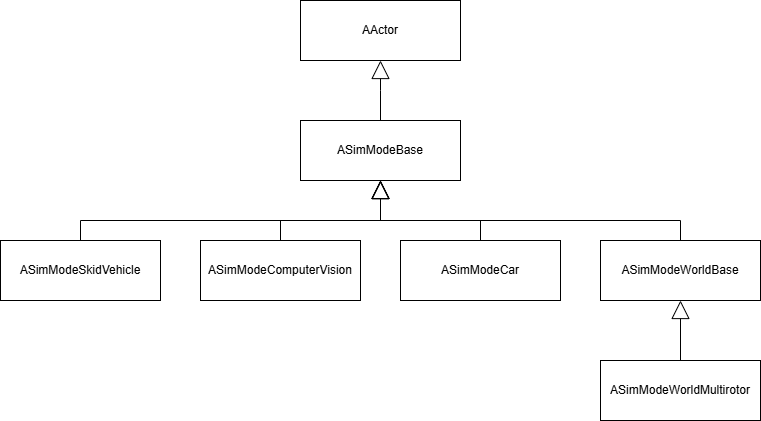
\includegraphics[width=0.7\textwidth]{graphics/simmode_hierarchy.png}
    \caption{\small UML Class Hierarchy for Cosys-AirSim Simulation Modes.}
    \label{fig:simmode_hierarchy}
\end{figure}
\noindent
The initialization process and interaction between the Unreal Engine and the AirSim plugin are illustrated in Figure \ref{fig:airsim_startup}.
\begin{figure}[H]
    \centering
    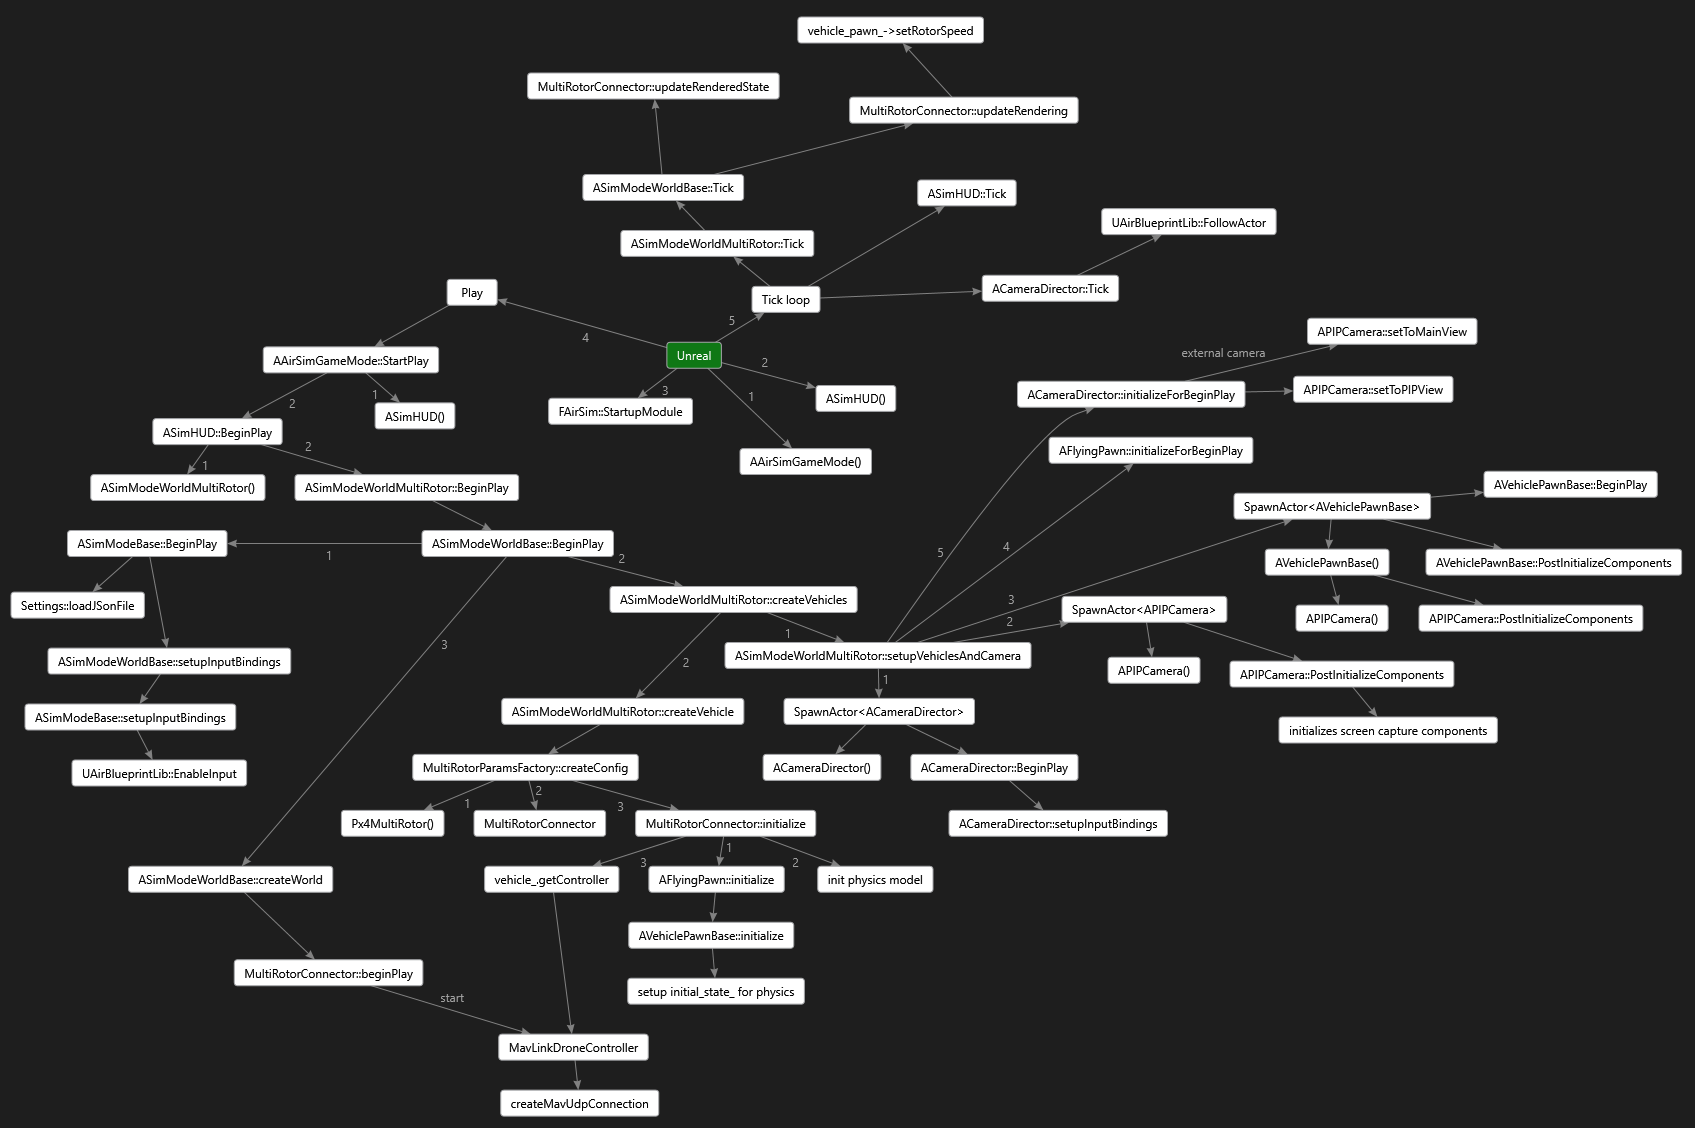
\includegraphics[width=0.7\textwidth]{graphics/airsim_startup.png}
    \caption{\small AirSim loading and invocation by Unreal Engine from the \href{https://airsim-fork.readthedocs.io/en/docs/code_structure.html}{official documentation}.}
    \label{fig:airsim_startup}
\end{figure}

\subsubsection{The Simulation API Bridge}
\noindent
This critical layer manages the bidirectional data flow between the core library and the rendering engine.

\begin{description}
    \item[\texttt{PawnSimApi}:] The primary mediator.  It subscribes to \texttt{pawn\_events} to catch Unreal collisions and frame ticks, while simultaneously implementing the \texttt{VehicleSimApiBase} from AirLib to update the vehicle's 3D transform (position and orientation) based on physics calculations.
    \item[Vehicle-Specific APIs:] Classes like \texttt{CarSimApi} and \texttt{MultirotorSimApi} extend  the base functionality to handle unique actuators, such as wheel rotation, suspension compression, or rotor blur effects, ensuring the visual representation matches the internal physical state.
\end{description}

\newpage

\section{Multidomain Extension}
\subsection{Overview}
\noindent
The base architecture of Cosys-AirSim, inherited from its predecessor Microsoft AirSim, was robust yet fundamentally limited by a strict single-domain paradigm. A simulation session could be configured to host either Unmanned Aerial Vehicles (UAVs) or Unmanned Ground Vehicles (UGVs), but never both simultaneously. This represented a severe bottleneck for modern robotics research, which increasingly relies on Heterogeneous Multi-Agent Systems (MAS) to solve complex real-world problems.\newline\newline
To bridge this critical gap, this project develops a comprehensive multidomain extension. Hence, this extension transitions Cosys-AirSim from a simple vehicle emulator into a holistic testing ground for advanced multi-agent coordination. At its core, the extension introduces a novel architectural component: the \texttt{SimModeWorldMultidomain} class. This specialized C++ module acts as an orchestrator within the Unreal Engine environment, capable of dynamically allocating dedicated communication ports and handling disparate vehicle physics models concurrently.\newline\newline
The impact of this development is relevant,  particularly within the realm of AI-powered robotics. By enabling an environment where aerial and ground vehicles coexist seamlessly, it unlocks entirely new experimental paradigms. For instance, it becomes possible to train reinforcement learning models where a drone acts as an "eye in the sky," streaming fused sensor data to an edge-AI algorithm that actively guides a ground rover through hazardous terrain. \newline

\subsubsection{Target Audience}
\noindent
The versatile nature of this environment caters to a broad spectrum of stakeholders, structured according to their level of engagement with the platform's core features:

\begin{description}
    \item[Primary Users:] include industrial and civil engineers focused on infrastructure inspection, construction, and cultural heritage preservation, as well as emergency response coordinators managing search and rescue missions.
    
    \item[Secondary Users:] encompass specialized sectors such as agricultural engineers exploring smart farming automation, as well as defense and security professionals who leverage controlled simulations to evaluate tactical coordination between autonomous aerial and ground units, and academic researchers advancing the field of cooperative robotics.
\end{description} 

\subsubsection{Example of Use Case: Torre dei Conti}
\noindent
In \textbf{industrial inspection and construction}, the extended Cosys-AirSim framework allows engineers to simulate the behaviour of UAVs and UGVs around fragile historical buildings, an application that could reduce the need for full human teams in potentially dangerous contexts. 
Given the delicate nature of such environments, it is crucial to minimize errors that could result in cultural losses or more severe consequences, as incidents like the partial collapse of Torre dei Conti (Rome, Nov~2025) \cite{torredeiconti} demonstrate. 
In these contexts, drones are already valuable tools (\href{https://roma.corriere.it/notizie/cronaca/25_novembre_09/torre-dei-conti-ecco-le-immagini-choc-dentro-il-monumento-quattro-piani-polverizzati-le-scale-sparite-d8165707-7645-470d-9343-b4c55e5dcxlk.shtml}{Corriere della Sera}), even though UAV–UGV configurations remain uncommon. 
The simulation focuses on assessing how robots move, sense, and coordinate in environments where structural stability is uncertain and even minor trajectory errors could exacerbate existing damage. 
By virtually testing flight paths, collision avoidance, take-off and landing procedures, and multi-robot cooperation, users can identify risky manoeuvres, communication blind spots, or areas with insufficient sensor coverage. This preparation helps refine mission logic, adjust autonomous behaviours, and design safer inspection strategies before approaching the real site, reducing overall risk.
\begin{figure}[H]
\centering
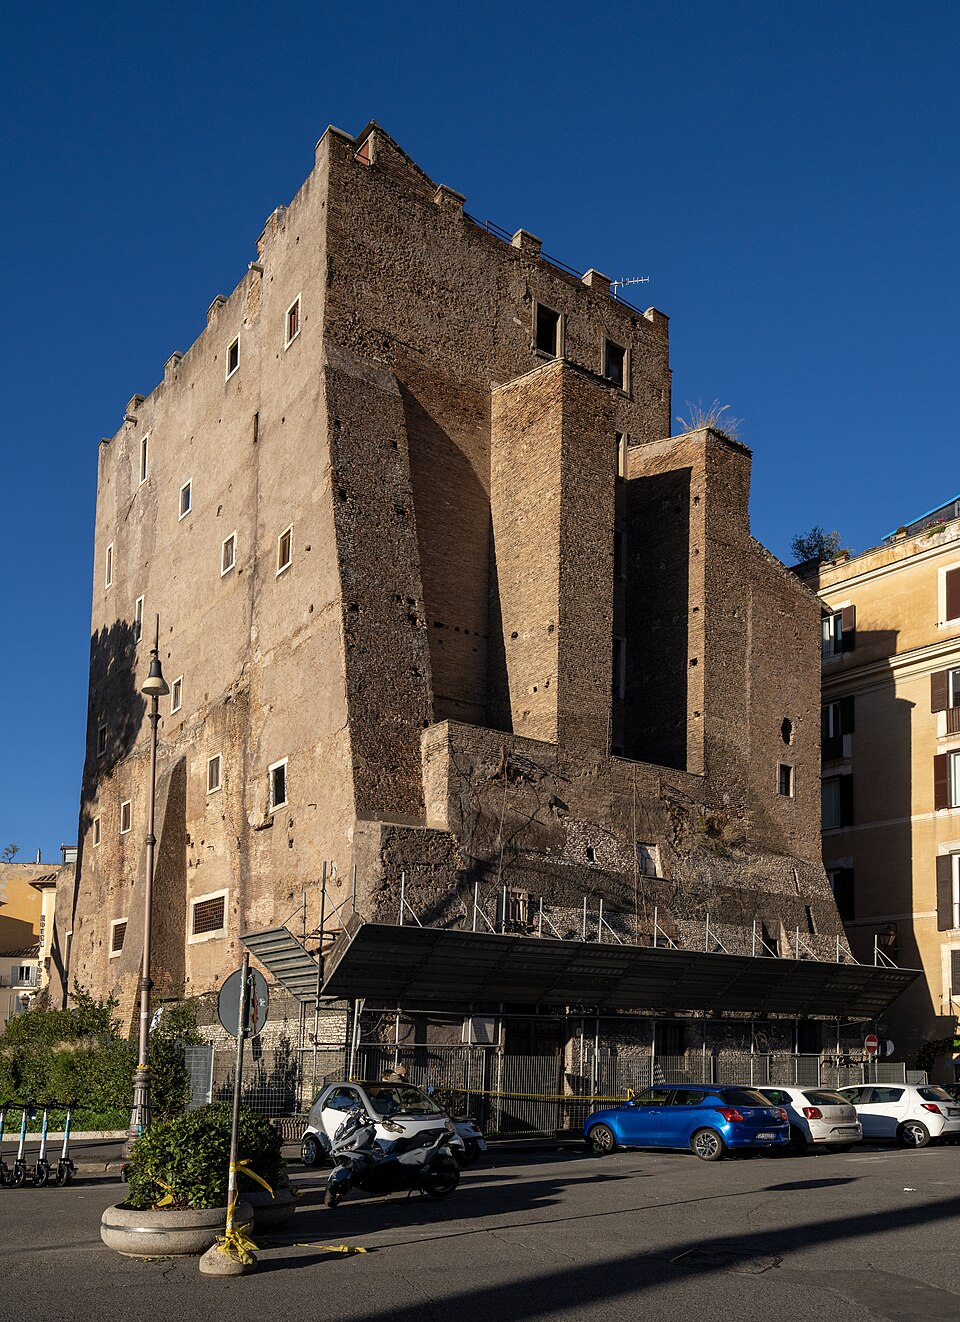
\includegraphics[width=0.3\textwidth]{graphics/torre_de_conti.jpg}
\caption{Torre de' Conti in its original state prior to the November 2025 collapse.}
\label{fig:torre_de_conti}
\end{figure}
\noindent

\subsection{Integration Steps}
\noindent
To integrate the Multidomain Extension, begin by cloning the repository: \newline\newline
\texttt{git clone <LINK\_TO\_FINAL\_REPO>}

\subsubsection{Step 1: Create the C++ Class in Unreal Engine}
\begin{enumerate}
    \item Launch the \texttt{.uproject} file (e.g., \texttt{Blocks.uproject}) that utilizes the Cosys-AirSim plugin.
    \item Initialize the class: 
    \begin{itemize}
        \item Navigate to \texttt{Tools} $\rightarrow$ \texttt{New C++ Class...}
        \item Select \texttt{All Classes}, search for \textbf{\texttt{SimModeWorldBase}}, and click \texttt{Next}.
    \end{itemize}
    \item Configure the files:
    \begin{description}
        \item[Name:] \texttt{SimModeWorldMultidomain}
        \item[Path:] \texttt{.../Plugins/AirSim/Source/Vehicles/Multidomain/}
    \end{description}
    \begin{figure}[H]
    \centering
    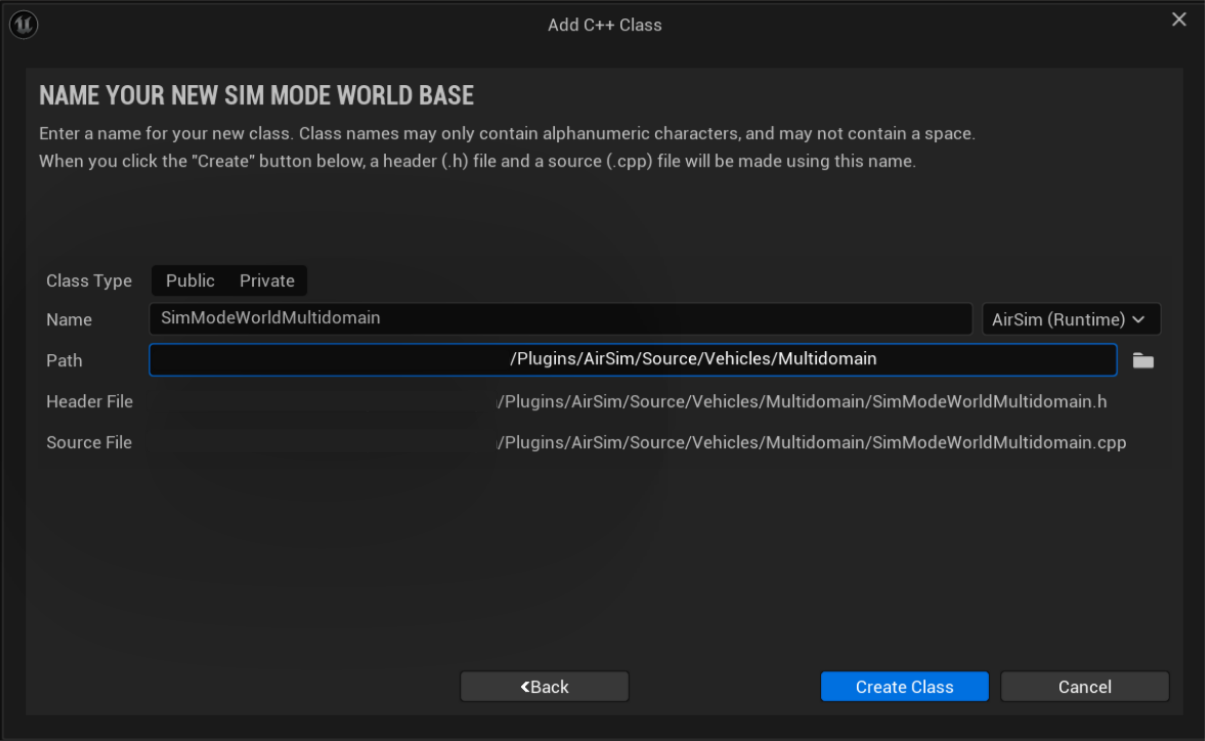
\includegraphics[width=0.7\textwidth]{graphics/new_class.png}
    \caption{\small Unreal Engine dialog showing the class name and destination path during extension integration.}
    \label{fig:ue_add_cpp_class_plugin}
    \end{figure}
    \item Click \texttt{Create Class} and wait for the \textit{Live Coding} notification to complete.
\end{enumerate}



\subsubsection{Step 2: File Replacement Registry}
\noindent
Replace the following existing files in your local directory with the modified versions from the cloned repository:

\begin{table}[H]
\centering
\small
\begin{tabular}{lll}
\toprule
\textbf{Directory Path (.../Plugins/AirSim/Source/)} & \textbf{Files to Replace} \\ \midrule
\texttt{AirLib/include/common/}        & \texttt{AirSimSettings.hpp} \\
\texttt{SimMode/}                      & \texttt{SimModeBase.*}, \texttt{SimModeWorldBase.*} \\
\texttt{SimHUD/}                       & \texttt{SimHUD.cpp} \\
\texttt{Vehicles/Car/}                 & \texttt{SimModeCar.*} \\
\texttt{Vehicles/Multidomain/}         & \texttt{SimModeWorldMultidomain.*} \\
\texttt{Vehicles/Multirotor/}          & \texttt{SimModeWorldMultirotor.*} \\
\texttt{Vehicles/ComputerVision/}      & \texttt{SimModeComputerVision.*} \\
\texttt{Vehicles/SkidVehicle/}         & \texttt{SimModeSkidVehicle.*} \\ \bottomrule
\end{tabular}
\end{table}

\subsubsection{Step 3: Clean and Rebuild Environment}
\begin{enumerate}[label=\alph*.]
     \item Navigate to \texttt{Plugins/AirSim/} and delete its specific \texttt{Binaries} and \texttt{Intermediate} folders.
    \item Delete the following folders from your project root: 
    \texttt{Binaries}, \texttt{Intermediate}, \texttt{Saved}, \texttt{DerivedDataCache}.
    \item Delete the existing \texttt{.sln} file from your project root.
    \item Right-click the \texttt{.uproject} file $\rightarrow$ \texttt{Show More Options} $\rightarrow$ \texttt{Generate Visual Studio project files}.
    \item Open the new \texttt{.sln}. Ensure the configuration is set to \textbf{\texttt{DevelopmentEditor}} on \textbf{\texttt{Win64}}. Press \texttt{F5} to build and launch the editor.
\end{enumerate}


\subsection{Implementation Details}

\subsubsection{Core Class Modifications}
\noindent
To support the new multidomain capabilities, the existing Cosys-AirSim class hierarchy for simulation modes was expanded. Figure \ref{fig:simmode_hierarchy_extended} illustrates this updated architecture, highlighting the addition of the \texttt{\seqsplit{ASimModeWorldMultidomain}} class and its specific position within the inheritance tree.
\begin{figure}[H]
    \centering
    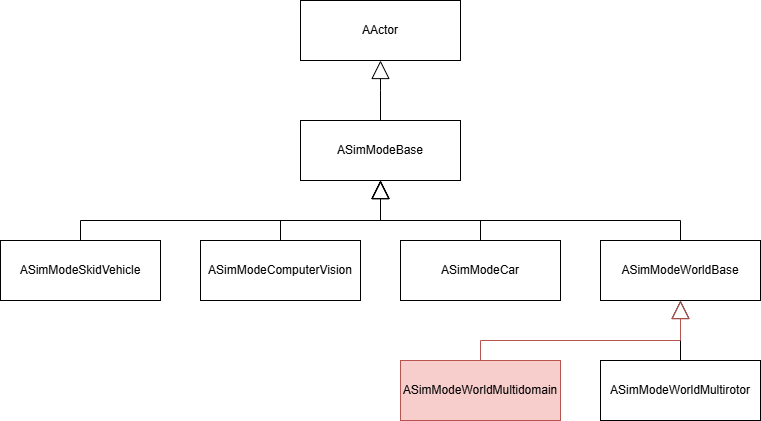
\includegraphics[width=0.7\textwidth]{graphics/simmode_hierarchy_extended.png}
    \caption{\small Modified UML Class Hierarchy for Cosys-AirSim Simulation Modes.}
    \label{fig:simmode_hierarchy_extended}
\end{figure}
\noindent
Table \ref{tab:simmode_modifications} provides a comprehensive summary of the modifications and additions implemented across the core files to support the multidomain simulation architecture.
\begin{longtable}{|p{0.22\textwidth}|p{0.28\textwidth}|p{0.42\textwidth}|}
    \caption{\small Summary of Modifications for Multidomain Simulation Modes.}
    \label{tab:simmode_modifications} \\
    \hline
    \textbf{Class} & \textbf{Method / Attribute} & \textbf{Modification Description} \\
    \hline
    \endfirsthead % This defines the header for the FIRST page
    
    \multicolumn{3}{c}{} \\
    \hline
    \textbf{Class} & \textbf{Method / Attribute} & \textbf{Modification Description} \\
    \hline
    \endhead % This defines the header for ALL SUBSEQUENT pages
    
    \hline
    \multicolumn{3}{r}{} \\
    \endfoot % This defines the footer for the bottom of the page when it breaks
    
    \hline
    \endlastfoot % This defines the footer for the very end of the table
    
    % --- AirSimSettings.hpp ---
    \texttt{\seqsplit{AirSimSettings}}
    & kSimModeTypeMultidomain
    & Creates a constant, file-specific pointer that points to the text `Multidomain'. \\ \cline{2-3}
    
    & \texttt{\seqsplit{loadCameraDirectorSetting}}
    & Defines the camera director follow distance (-8) and Z-position (-3) for Multidomain simulation mode. \\ \cline{2-3}
    
    & \texttt{\seqsplit{loadClockSettings}}
    & Sets clock type to \texttt{SteppableClock} unless a PX4 enabled vehicle is present (which triggers \texttt{ScalableClock}). \\ \cline{2-3}
    
    & \texttt{\seqsplit{createDefaultSensorSettings}}
    & Specifies default sensors (IMU, magnetometer, GPS, barometer) for Multidomain mode. \\ \cline{2-3}
    
    & \texttt{\seqsplit{loadCoreSimModeSettings}}
    & Enforces "FastPhysicsEngine" as the default physics engine if none is specified in settings. \\ \cline{2-3}
    
    & \texttt{\seqsplit{createDefaultVehicle}}
    & Generates a default drone and a default car if Multidomain mode is selected and no vehicles are specified. \\ 
    \hline
    
    % --- SimModeBase ---
    \texttt{\seqsplit{ASimModeBase}}
    & \texttt{createApiServer} 
    & Returns a dynamic array of smart pointers. \\ \cline{2-3}
    
    & \texttt{api\_servers\_} \newline (replacing \texttt{api\_server\_})
    & Refactored from a single smart pointer to multiple smart pointers holding multiple objects. \\ \cline{2-3}
    
    & \texttt{pawn\_to\_vehicle\_map} 
    & Added map data structure relating pawn pointers to their vehicle types. \\ \cline{2-3}

    & \texttt{addPawnToMap} 
    & Added method to insert entries into the tracking map. \\ \cline{2-3}
    
    & \texttt{getVehicleType} 
    & Added method returning the vehicle type string from the map (or an empty string if not found). \\
    \hline

    % --- SimModeWorldBase ---
    \texttt{\seqsplit{ASimModeWorldBase}}
    & \texttt{initializeForPlay} 
    & Established a bifurcated physics pipeline: drones use AirSim's \texttt{\seqsplit{PhysicsWorld}}, while cars use Unreal Engine's native physics. \\ \cline{2-3}

    & \texttt{registerPhysicsBody} 
    & Restricted custom physics registration to dynamically spawned drones, preserving the bifurcated architecture. \\ \cline{2-3}

    & \texttt{Tick} 
    & Separated state updates by physics domain to prevent thread conflicts between custom and native physics. \\ \cline{2-3}

    & \texttt{reset} 
    & Implemented independent resets for the custom physics world (drones) and Unreal Engine's native physics (cars). \\ 
    \hline

    % --- SimModeSkidVehicle ---
    \texttt{\seqsplit{ASimModeSkidVehicle}}
    & \texttt{createApiServer} 
    & Modified to return a dynamic array of smart pointers instead of a single smart pointer. \\ 
    \hline

    % --- SimModeWorldMultirotor ---
    \texttt{\seqsplit{ASimModeWorldMultirotor}} 
    & \texttt{createApiServer} 
    & Modified to return a dynamic array of smart pointers instead of a single smart pointer. \\ 
    \hline
    
    % --- SimModeComputerVision ---
    \texttt{\seqsplit{ASimModeComputerVision}}
    & \texttt{createApiServer} 
    & Modified to return a dynamic array of smart pointers instead of a single smart pointer. \\  \cline{2-3}
    
    & \texttt{\seqsplit{isPaused}} \& \texttt{\seqsplit{pause}}
    & Overridden to use Unreal's \texttt{\seqsplit{UGameplayStatics}} to safely check, stop, or resume simulation execution. \\ 
    \hline
    
    % --- SimModeCar ---
    \texttt{\seqsplit{ASimModeCar}}
    & \texttt{createApiServer} 
    & Modified to return a dynamic array of smart pointers instead of a single smart pointer. \\  \cline{2-3}
    
    & \texttt{\seqsplit{isPaused}} \& \texttt{\seqsplit{pause}} 
    & Overridden to use an internal variable (\texttt{\seqsplit{current\_clockspeed\_}}) to pause, or resume by scaling time in Unreal. \\ 
    \hline
    
    % --- SimModeWorldMultidomain ---
    \texttt{\seqsplit{ASimModeWorldMultidomain}} \newline (New Class)
    & \texttt{BeginPlay} \& \texttt{EndPlay} 
    & Initializes the physics world, and safely stops the physics engine before Unreal dismantles the world. \\ \cline{2-3}
    
    & \texttt{setupClockSpeed} 
    & Configures internal timing, dynamically scaling the physics control loop to allow time manipulation safely. \\ \cline{2-3}
    
    & \texttt{createApiServer} 
    & Opens two separate RPC servers simultaneously: port 41451 (Multirotors) and port 41452 (Cars). \\ \cline{2-3}
    
    & \texttt{getExistingVehiclePawns} 
    & Scans environment for drones and cars, pushing them to the internal tracking map with type flags. \\ \cline{2-3}
    
    & \texttt{isVehicleTypeSupported}
    & Whitelists \texttt{\seqsplit{kVehicleTypeSimpleFlight}} and \texttt{\seqsplit{kVehicleTypePhysXCar}}. \\ \cline{2-3}
    
    & \texttt{\seqsplit{getVehiclePawnPathName}}
    & Acts as a fallback for spawning default blueprints. \\ \cline{2-3}
    
    & \texttt{getVehiclePawnEvents} \newline \texttt{getVehiclePawnCameras} 
    & Retrieves specific event handlers and camera attachments for a given pawn. \\ \cline{2-3}
    
    & \texttt{initializeVehiclePawn} \newline \texttt{createVehicleSimApi} 
    & Triggers domain-specific initializations and instantiates core simulation APIs based on the vehicle domain. \\
    \hline

    % --- SimHUD ---
    \texttt{ASimHUD} 
    & \texttt{getSimModeFromUser} 
    & Added a message to the initial sequence dialogue prompting the user to choose a multidomain or monodomain simulation. \\ \cline{2-3}
    
    & \texttt{createSimMode} 
    & Spawns the \texttt{ASimModeWorldMultidomain} actor based on user choice or settings. \\ 
    \hline
    
\end{longtable}

\subsubsection{Development Environment \& Toolchain}
\noindent
The development and execution of the simulation environment for the drone and car multi-agent system relied on several key software tools and libraries. Below is the list of the primary tools utilized:

\begin{itemize}
    \item \textbf{Technologies \& Software:} Visual Studio Community 2022, Git, Github, LaTeX
    \item \textbf{Platforms:} Desktop Platforms
    \item \textbf{Programming Languages:} C++, Python
    \item \textbf{Frameworks:} Unreal Engine 5.5.4, Cosys-AirSim v3.3
    \item \textbf{Database:} None required
    \item \textbf{Cloud:} None required
\end{itemize}
\noindent
The following section details the specific roles and implementation of each tool within the project workflow:

\begin{enumerate}
    \item \textbf{Cosys-AirSim (v3.3.0)}: An advanced, open-source simulator for autonomous vehicles, developed as an extension of Microsoft AirSim by the Cosys-Lab at the University of Antwerp. It is specifically designed for research-focused simulations, offering enhanced support for sensors and multi-agent systems within Unreal Engine 5.5.
    \item \textbf{Unreal Engine 5.5.4}: A high-performance 3D creation tool used to build the simulation environment. It provides the physics engine (Chaos Physics), photorealistic rendering, and the overall framework for vehicle interaction and environmental dynamics.
    \item \textbf{Python}: The primary programming language used to develop the control scripts.
    \item \textbf{C++}: The core programming language used by Unreal Engine and for the development of the Cosys-AirSim plugin.
    \item \textbf{cosysairsim package}: The official Python client wrapper for the simulation. It provides a Python interface to AirLib, facilitating communication between external control scripts and the Unreal Engine environment via RPC (Remote Procedure Call).
    \item \textbf{Visual Studio Community 2022}: The Integrated Development Environment (IDE) used for building the C++ components of the plugin and managing the Unreal Engine project dependencies.
    \item \textbf{\LaTeX}: The document preparation system used for the professional typesetting of this project report.
\end{enumerate}

\subsection{Scope and Limitations}
\noindent
While our implementation successfully enables the concurrent simulation of multiple vehicle domains, certain technical limitations remain due to the project's development timeline. These constraints are not viewed as failures but rather as opportunities for future work to further enhance the framework:
\begin{itemize}    
   \item \textbf{Dynamic Camera Switching:} A significant limitation is the inability to use any built-in mechanism to dynamically switch the main camera view between different vehicles in the Unreal Engine scene during a live simulation. While it is possible to bind the three available Picture-in-Picture (PiP) subwindows to vehicles in \texttt{\seqsplit{settings.json}} before starting, this is strictly limited to three additional vehicles. Furthermore, these windows are quite small, which restricts the user's visibility and makes it difficult to monitor individual agents if they move far apart or encounter unexpected issues.
    
    \item \textbf{Expanded Vehicle Support:} Currently, supported vehicle types are limited to \texttt{\seqsplit{kVehicleTypePhysXCar}} and \texttt{\seqsplit{kVehicleTypeSimpleFlight}}. Expanding operational support to include additional domains and vehicle types, such as \texttt{kVehicleTypeArduRover}, would represent a significant enhancement.
\end{itemize}

\newpage

\section{Results}
%Examples and Test control scripts 
\noindent
The implementation was successfully validated using multiple demonstration scripts.
The primary objective of these tests was to ascertain whether the framework could seamlessly spawn, initialize, and control both drones and cars simultaneously within the exact same Unreal Engine 5 instance, without triggering the core engine conflicts that plagued the baseline single-domain Cosys-AirSim.\newline\newline
The test \texttt{\seqsplit{multi\_agent\_drone\_car}} instantiates two independent client objects from the Cosys-AirSim Python API. The extension allows these clients to bind to dedicated Localhost API server ports: port 41451 is exclusively assigned to handle the multirotor control signals, while port 41452 was bound to the car commands.\newline
During the active execution phase, both vehicles achieve real-time, asynchronous operation. The script commands \texttt{Drone1} to arm, execute an automated takeoff sequence (\texttt{takeoffAsync}), and perform trajectory tracking via \texttt{moveToPositionAsync}. In parallel, \texttt{Car1} is simultaneously supplied with continuous \texttt{CarControls} inputs (throttle set to 0.5, steering set to 0.5), initiating a curved forward movement. \newline\newline
The test \texttt{car\_hit\_drone} specifically validates the physical interaction and collision detection between heterogeneous agents. In this scenario, \texttt{Drone1} is placed in a stationary state on the ground, acting as a passive obstacle. \texttt{Car1} is then commanded to move forward at full throttle directly towards the UAV. The results demonstrate that the Unreal Engine physics engine, as extended by the framework, correctly processes the collision: the car physically impacts the drone and reflects off it, confirming that the separate API domains do not isolate the agents from the global physics environment.\newline\newline
The test \texttt{cars\_intersection\_crash} evaluates multi-vehicle interaction within the ground domain. Three cars are instantiated: two navigating along a horizontal axis and one along a vertical axis, creating a four-way intersection scenario. The script commands all vehicles to accelerate simultaneously towards the center. Upon impact, the framework accurately simulates the transfer of momentum and torque, resulting in realistic physical behaviors such as vehicle spinning and lateral displacement post-collision, further validating the robustness of the multi-agent physics integration.\newline\newline
The scenario \texttt{drone\_hit\_car} provides a dual-domain collision test where the UAV acts as the kinetic agent. The script initializes \texttt{Car1} in a braking state and calculates its vertical position to allow \texttt{Drone1} to lock its altitude precisely to the car's chassis level. Upon impact, the framework demonstrates consistent collision geometry: the drone is physically repelled by the car's collider, reflecting the impact. While the stationary car's displacement is negligible due to the significant mass differential and simulated tire friction, the test confirms that the UAV's flight controller and the global physics engine successfully register the collision event across the heterogeneous multi-agent setup.\newline\newline
The test \texttt{drones\_rapid\_cross} focuses on high-velocity multi-agent coordination within the aerial domain. Three UAVs are programmed to perform a synchronized, high-speed crossing maneuver at the same altitude. During the execution, the system maintains stable control over all three drones until a collision occurs between two of them. The results show that the framework correctly detects the high-speed impact; the involved drones become physically interlocked, demonstrating that the physics engine accurately handles complex mesh-to-mesh interactions even at significant relative velocities.\newline\newline
The \texttt{full\_chaos} test serves as a stress and stability benchmark for the multi-port API extension. This scenario instantiates a large number of heterogeneous agents, both cars and drones, and commands them to move in divergent, semi-random directions. The simulation results confirm that the framework can simultaneously handle multiple physics-driven interactions: some vehicles successfully navigate open spaces while others collide with static environment geometry (e.g., buildings, walls). Throughout this high-load phase, the communication between the distributed API servers (multirotor and car) remains synchronized, with no observed latency spikes or command drops, validating the scalability of the proposed extension.\newline\newline
The \texttt{many\_vehicles} scenario validates the system's ability to manage a coordinated fleet of heterogeneous agents. In this test, the framework controls two UAVs and two UGVs simultaneously, while other inert vehicles are present in the environment map. The script executes a synchronized escort pattern where both drones and cars advance in a forward trajectory. The telemetry logs demonstrate that the framework maintains independent and precise control over each specific vehicle instance (e.g., \texttt{Drone1}, \texttt{Drone2}, \texttt{Car1}, \texttt{Car2}) across their respective API ports, ensuring that the presence of multiple active agents does not lead to command crosstalk or resource exhaustion within the Unreal Engine instance.\newline\newline
The final test, \texttt{swarm\_takeoff}, examines the synchronization of multi-agent aerial maneuvers. In this scenario, three drones are commanded to perform a simultaneous takeoff, followed by a rapid vertical ascent to an altitude of 15 meters. The results confirm that the framework can broadcast and synchronize identical high-level commands across multiple UAV instances without jitter or significant timing offset, validating the system's capability for swarm-based research.\newline\newline
The results are definitively positive. Polling the \texttt{getCarState} and \texttt{getMultirotorState} functions confirm that the vehicles achieve stable initialization and control. Both the UAV and UGV successfully coexist and navigate their distinct physical domains, thereby thoroughly fulfilling the primary objective of the extension. While the framework demonstrates high functional reliability across all tested scenarios, future work will focus on optimizing long-duration stability under complex collision environments to ensure maximum simulation uptime.

\newpage

\section{Conclusion}
\noindent
The development of the multi-domain extension for Cosys-AirSim marks a significant milestone in expanding the simulation capabilities of the Unreal Engine 5 framework. By successfully modifying the core architecture to accommodate different vehicle classes dynamically, this project bridged the gap between single-domain operations and heterogeneous multi-vehicle environments. 
The validation tests clearly demonstrate the stability of assigning isolated communication interfaces natively, allowing both unmanned aerial vehicles (UAVs) and unmanned ground vehicles (UGVs) to operate concurrently within the same ecosystem.\newline
This enhancement provides researchers, engineers, and developers with a vastly expanded, comprehensive testing ground. The ability to natively simulate cooperative operations unlocks entirely new avenues for testing advanced Artificial Intelligence algorithms, multi-agent path planning, and complex reinforcement learning models in a risk-free, high-fidelity virtual world. Ultimately, this work establishes a robust and critically needed foundation for next-generation multi-agent robotics simulations, empowering the scientific community to innovate safely and effectively before real-world deployment.

\newpage

\bibliographystyle{plain}
\bibliography{refs}
\nocite{*}
\end{document}
